\documentclass[12pt,a4paper]{article}
\usepackage[margin=21mm,headheight=16pt]{geometry}
\usepackage[T1]{fontenc}
\usepackage{lmodern,microtype,amsmath,amssymb,booktabs,tabularx,graphicx}
\usepackage{enumitem,fancyhdr,caption,placeins}
\usepackage[colorlinks=true,urlcolor=blue,linkcolor=black,citecolor=black]{hyperref}
\setlength{\parindent}{0pt}
\setlength{\parskip}{5pt}
\setlength{\emergencystretch}{2em}
\setlist{nosep,leftmargin=1.4em}
\captionsetup{font=small,labelfont=bf}
\renewcommand{\topfraction}{0.9}
\renewcommand{\bottomfraction}{0.85}
\renewcommand{\textfraction}{0.08}
\renewcommand{\floatpagefraction}{0.85}
\pagestyle{fancy}
\fancyhf{}
\fancyhead[L]{\small CSE 516 -- Milestone 3}
\fancyhead[R]{\small Group 4}
\fancyfoot[C]{\thepage}
\newcommand{\E}{\mathbb E}
\newcommand{\Var}{\operatorname{Var}}
\newcommand{\N}{\mathcal N}
\newcommand{\code}[1]{\texttt{#1}}
\begin{document}
\begin{titlepage}
\thispagestyle{empty}
{\large\bfseries 1. Title Page}\par
\vspace{17mm}
\begin{center}
{\Large\bfseries Ahmedabad University}\par
\vspace{3mm}
{\Large\bfseries CSE 516 -- Probabilistic Graphical Models}\par
\vspace{5mm}
{\large Milestone 3: Results and Analysis}\par
\vspace{15mm}
{\fontsize{18}{22}\selectfont\bfseries Bayesian Personalized Recommendation using\\[3pt]
Latent Trait Models \& Expectation Propagation}\par
\vspace{5mm}
{\large\bfseries Category: Theoretical AI}\par
\vspace{2mm}
{\large\bfseries Group 4}\par
\vspace{10mm}
\renewcommand{\arraystretch}{1.18}
\begin{tabular}{ll}\toprule
\textbf{AU ID} & \textbf{Student Name}\\\midrule
AU2440170 & Jyotier Vithalani\\
AU2440234 & Tanmay Kanani\\
AU2440259 & Ansh Chaudhari\\
AU2440178 & Shlok Shah\\
AU2440221 & Het Patel\\\bottomrule
\end{tabular}
\vfill
\textbf{GitHub Repository}\par
\vspace{2mm}
{\small\url{https://github.com/Jyotier2006/M2_g4_th_apl_recommend-sys_team}}\par
\vspace{10mm}
\textbf{Submission Date:} 4 November 2026\par
\vspace{4mm}
\end{center}
\end{titlepage}
\setcounter{page}{1}
\setcounter{section}{1}

\section*{Abstract}
We extend the existing M2 study of a restricted static Matchbox recommender
with systematic full-data experiments and an explicit Gaussian Markov movie
prior. Across five MovieLens 1M splits, ADF, EP5 and EP10 achieve expected-rating
RMSE $0.8977\pm0.0035$, $0.8643\pm0.0037$ and $0.8548\pm0.0029$.
GMRF-MAP achieves $0.8499\pm0.0023$, but its matched graph-free MAP baseline
already reaches $0.8506\pm0.0021$: the isolated graph gain is modest.
Paired user-bootstrap intervals support a reduction in four of five splits;
one includes zero. Repeated EP improves NLL while worsening ECE, and changing
observation noise does not uniformly improve probability quality.
Missing-data, corrupted-label, graph-density, metadata and cold-start tests
probe robustness. Exact Gaussian and numerical quadrature diagnostics expose
what the approximations preserve and lose. These results position the project
as an inference and regularization study, not a full Matchbox/PreRec
reproduction or a state-of-the-art claim.

\section{Problem and cumulative progress from M1/M2}
Sparse user--item ratings leave uncertainty about both preferences and item
characteristics. A latent-trait graphical model shares evidence across ratings
through common user and item parameters, while Bayesian learning retains
uncertainty about those parameters. Our original theoretical question remains:
\emph{how do ADF and repeated EP differ in predictive quality, uncertainty,
computation and memory?} M3 adds: \emph{does an explicit movie Markov prior
improve a matching matrix-factorization model, and under which conditions?}

This is an update of the M2 report. The project identity, latent-trait model,
EP/VMP equations and validation foundation are retained. M3 expands the
benchmark to five seeds, adds MAP and graph ablations, studies both assumed
noise and corrupted observations, and replaces the preliminary conclusion
with evidence from measured runs. The earlier synthetic offline demo is not
used as MovieLens evidence. The original M2 result files remain separately
labelled for provenance.

The work retains the Theoretical AI track with recommendation as its benchmark.
The new graph is constructed from training similarities, not learned through
causal structure discovery. User-specific thresholds and temporal dynamics
remain outside the implemented scope. We compare several meaningful approaches;
we do not claim to test every possible PGM algorithm.

\section{Probabilistic representation}
For user $u$ and item $i$, let $s_u,t_i\in\mathbb R^K$ denote latent traits and
$b_u,b_i$ denote biases. For each observed pair $(u,i)\in\mathcal D$,
\begin{align}
z_{uik}&=s_{uk}t_{ik}, &
a_{ui}&=\mu+b_u+b_i+\sum_{k=1}^{K}z_{uik},\label{eq:affinity}\\
y_{ui}\mid a_{ui}&\sim\N(a_{ui},\beta^2), &
R_{ui}=r&\iff c_{r-1}<y_{ui}\leq c_r.\label{eq:ordinal}
\end{align}
Only the rating is observed. The cuts are
$c=(-\infty,1.5,2.5,3.5,4.5,+\infty)$; $\mu$ is the training mean, treated as
fixed. Independent priors are
\begin{equation}
s_{uk}\sim\N(m^0_{uk},0.25),\quad t_{ik}\sim\N(n^0_{ik},0.25),\quad
b_u,b_i\sim\N(0,1).
\end{equation}
Trait prior means are sampled once from $\N(0,0.1^2)$ using the run seed. This
breaks bilinear sign symmetry without using held-out ratings.

With $\Theta=(S,T,b_U,b_I)$, the joint factorization is
\begin{equation}
\begin{aligned}
p(\Theta,Z,A,Y,R)=p(\Theta)\prod_{(u,i)\in\mathcal D}
&\left[\prod_k\delta(z_{uik}-s_{uk}t_{ik})\right]\\[-2pt]
&\times\delta\!\left(a_{ui}-\mu-b_u-b_i-\sum_k z_{uik}\right)\\[-2pt]
&\times\N(y_{ui};a_{ui},\beta^2)
\mathbf1\{c_{R_{ui}-1}<y_{ui}\le c_{R_{ui}}\}.
\end{aligned}\label{eq:joint}
\end{equation}

\begin{figure}[!htbp]\centering
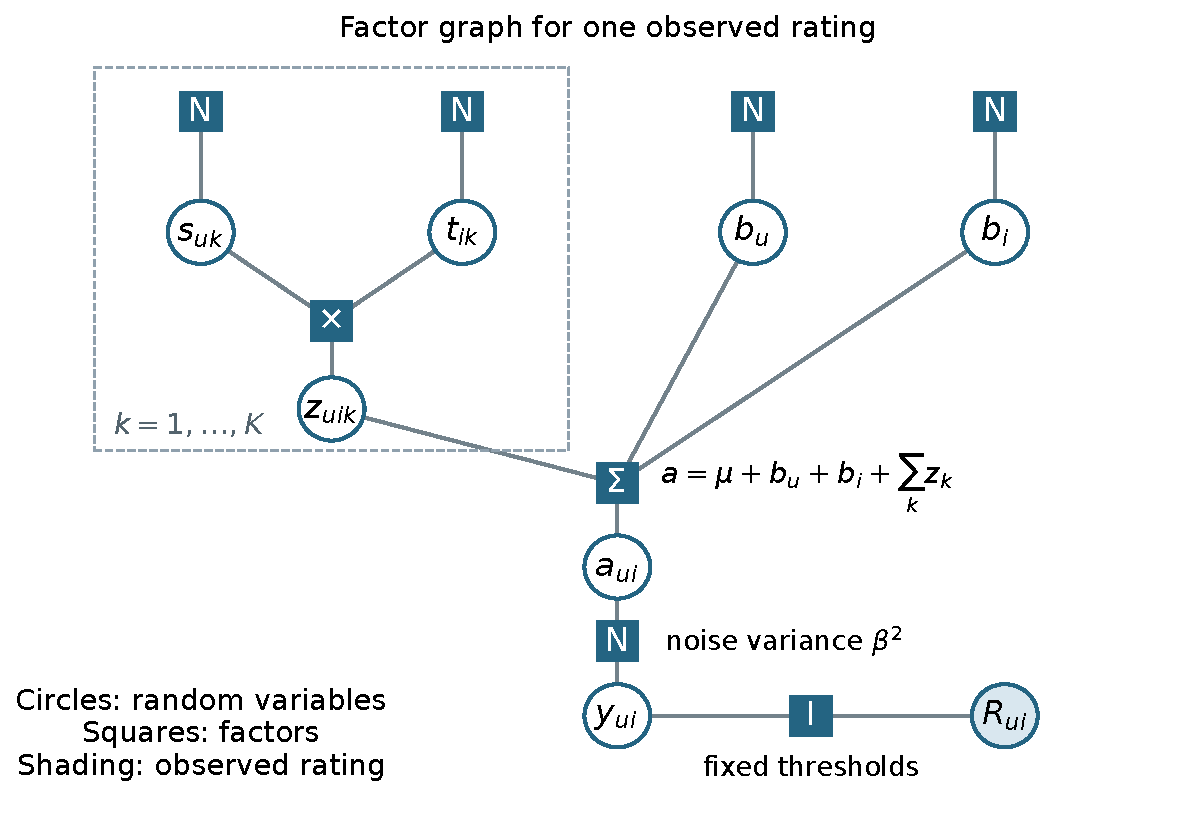
\includegraphics[width=\linewidth]{figures/factor_graph.pdf}
\caption{Factor graph for one rating. The plate repeats the trait product;
user/item variables are shared across all corresponding ratings. Edges connect
variables to the factors that depend on them.}
\label{fig:graph}
\end{figure}

Prior factors regularize parameters; products express compatibility; the sum
adds biases; Gaussian noise captures residual variation; and the interval
factor converts a continuous score into a rating. The preserved M2 reference includes a
concrete variable/factor/edge specification in \code{graph\_instance.json}.

Ratings are conditionally independent given all relevant parameters. Ratings
sharing a user or item are generally dependent after marginalization. Independent
priors do not imply independent posterior parameters: the factorized Gaussian
posterior is an approximation. The model assumes stationary preferences and does
not model why a movie was rated or identify causal effects.

\section{Learning and inference}
\subsection{Posterior learning and prediction query}
Training approximates $p(\Theta\mid R_{\mathcal D})$ by a product of univariate
Gaussians, storing precision $\lambda=1/v$ and weighted mean $\eta=m/v$.
Thresholds remain fixed; noise and prior variances are fixed within a run and varied in the M3 sensitivity experiments. Prediction computes
$p(R_{ui}=r\mid R_{\mathcal D})$ for an unobserved pair.

Under the factorized approximation, product moments are
\begin{align}
M_k&=\E[s_kt_k]=m_{s_k}m_{t_k},\\
V_k&=\Var(s_kt_k)=v_{s_k}v_{t_k}+v_{s_k}m_{t_k}^{2}+v_{t_k}m_{s_k}^{2}.
\end{align}
\begin{samepage}
Set $m_y=\mu+m_{b_u}+m_{b_i}+\sum_kM_k$ and
$v_y=\beta^2+v_{b_u}+v_{b_i}+\sum_kV_k$. Approximating the score as Gaussian gives
\begin{equation}
\widehat p_r=\Phi\!\left(\frac{c_r-m_y}{\sqrt{v_y}}\right)
-\Phi\!\left(\frac{c_{r-1}-m_y}{\sqrt{v_y}}\right),\qquad
\widehat R=\sum_{r=1}^{5}r\widehat p_r.\label{eq:prediction}
\end{equation}
The moments are exact under the factorized $q$; the Gaussian score approximation
is additional. Probabilities use a $10^{-15}$ numerical floor and renormalization.
\end{samepage}

\subsection{Local hybrid EP/VMP update}
Exact posterior inference is intractable at this scale because bilinear products
and ordinal observations couple many parameters. Following Matchbox~\cite{stern2009},
we use VMP at products and EP or exact Gaussian messages elsewhere. A local loop
alternates forward moments, ordinal moment matching and reverse messages,
reconstructing marginals from a fixed cavity and the current message.

For an incoming score $\N(m,v)$, define $\alpha=(c_{r-1}-m)/\sqrt v$,
$\gamma=(c_r-m)/\sqrt v$ and $Z=\Phi(\gamma)-\Phi(\alpha)$. Truncated moments are
\begin{align}
\widehat m&=m+\sqrt v\,\frac{\phi(\alpha)-\phi(\gamma)}{Z},\\
\widehat v&=v\left[1+\frac{\alpha\phi(\alpha)-\gamma\phi(\gamma)}{Z}
-\left(\frac{\phi(\alpha)-\phi(\gamma)}{Z}\right)^2\right].
\end{align}
Gaussian division yields $\lambda_o=\widehat v^{-1}-v^{-1}$ and
$\eta_o=\widehat m/\widehat v-m/v$. Write the outgoing Gaussian as
$\N(y;m_o,v_o)$. Reverse propagation to product $z_k$ gives
\begin{align}
d_k&=m_o-\mu-m^{\setminus n}_{b_u}-m^{\setminus n}_{b_i}-\sum_{\ell\ne k}M_\ell,\\
w_k&=v_o+\beta^2+v^{\setminus n}_{b_u}+v^{\setminus n}_{b_i}+\sum_{\ell\ne k}V_\ell.
\end{align}
The VMP message to $s_k$ is
\begin{equation}
\lambda_{f\to s_k}=\frac{\E[t_k^2]}{w_k},\qquad
\eta_{f\to s_k}=\frac{d_k\E[t_k]}{w_k},\quad
\E[t_k^2]=v_{t_k}+m_{t_k}^2.
\end{equation}
The item update is symmetric. A bias receives the analogous Gaussian sum
message with its own cavity term omitted. Product moments use current local
marginals; bias inputs remain cavities. Local damping is 0.7, with at most
10 iterations and an absolute mean/variance change tolerance of $10^{-4}$.

\subsection{ADF versus repeated EP}
EP caches a Gaussian site per rating. For each touched scalar parameter,
\begin{equation}
\lambda=\lambda_0+\sum_n\lambda_n,\quad \eta=\eta_0+\sum_n\eta_n;
\qquad
\lambda^{\setminus n}=\lambda-\lambda_n,\quad
\eta^{\setminus n}=\eta-\eta_n.\label{eq:cavity}
\end{equation}
An EP pass visits the fixed training order, subtracts the old site's natural
parameters, runs the local update, and replaces that site. The replacement is
damped with weight 1 on pass one and 0.5 thereafter.

ADF processes each rating once and discards its site. Thus EP's first pass
matches ADF under identical priors and order. Replaying ADF without cavity
removal would double-count evidence. Our ADF interface rejects a second pass.
Five or ten EP passes are computational budgets, not proof of convergence.

\section{M3 extension: an explicit Markov movie network}
\subsection{What changed, and why it might help}
The M2 latent-trait model already is probabilistic. Its independent movie priors,
however, do not explicitly connect similar movies. M3 adds a separate Gaussian
Markov random field (GMRF) prior to a matrix-factorization model. An undirected
edge encourages two movies' latent vectors to remain similar. This can reduce
estimation variance when ratings are sparse or unreliable, but a misleading or
overly strong edge can introduce bias. Improvement is a hypothesis to test,
not a property guaranteed by the word ``Markov.''

The new model uses maximum a posteriori (MAP) estimation by alternating block
minimization. It does not add graph messages to the original EP implementation.
Consequently, comparing GMRF-MAP with EP changes both the prior and the fitting
method/likelihood. The controlled graph ablation is \textbf{GMRF-MAP versus
MF-MAP with $\gamma=0$}, sharing the data, initialization, regularization,
training budget and validation rules.

\subsection{Building the graph from available evidence}
\label{sec:graphconstruction}
For each split, the graph is constructed from training ratings and fixed movie
genres only. Five alternating regularized bias updates estimate $\mu,b_u,b_i$;
their residuals are $e_{ui}=R_{ui}-\mu-b_u-b_i$. Each movie's sparse residual
column is normalized. Positive residual cosine similarities are multiplied by
$n_{ij}/(n_{ij}+20)$, where $n_{ij}$ is the number of common training users;
similarities based on fewer than five common users are set to zero.

Genres are represented by an 18-dimensional multi-hot vector, normalized to
unit length before computing genre cosine similarity. Default affinities mix
90\% residual similarity and 10\% genre similarity. Each movie retains its top
20 positive neighbours; ties use mapped movie IDs. The union is symmetrized
using the maximum of the two directed weights, so final degrees can exceed 20.
If $A$ denotes this symmetric affinity, $W=D_A^{-1/2}AD_A^{-1/2}$.
We then recompute $D_{ii}=\sum_jW_{ij}$ and set $L=D-W$.
The diagonal of $W$ is zero. This is a deterministic similarity construction,
not causal discovery or recovery of a known true graph. Across the five main
splits, the graph has 56,408--56,575 undirected movie edges (mean 56,508),
mean degree 30.50, density 0.823\%, and no isolated movie nodes. These are
representation statistics, not edge-recovery accuracy. Because $W$ is
estimated from training ratings, this is a data-dependent, empirical-Bayes-style
regularization construction. We condition on the resulting $W$ and do not
propagate uncertainty about its edges.

\begin{figure}[!htbp]\centering
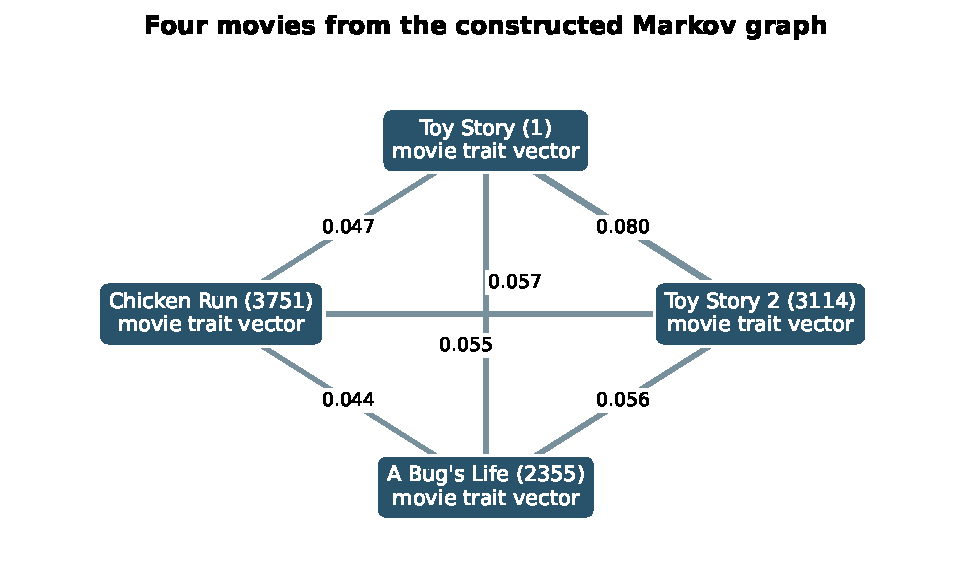
\includegraphics[width=.92\linewidth]{../../Results/analysis/plots/movie_subgraph.pdf}
\caption{Actual seed-42 subgraph: Toy Story and its three strongest neighbours.
Node labels give titles and raw MovieLens IDs; displayed edge labels are the
normalized weights. Each node represents a movie's latent vector; each edge
induces the pairwise factor in Equation~\ref{eq:gmrfprior}. The full graph has
many other neighbours. Similarity is not a causal claim.}
\end{figure}

\subsection{Factors, conditional independence and MAP objective}
With $Q_i\in\mathbb R^K$ for movie $i$, the movie prior is
\begin{align}
p(Q\mid W)&\propto
 \prod_i \exp\!\left(-\frac{\lambda}{2}\|Q_i\|^2\right)
 \prod_{\{i,j\}\in E}\exp\!\left(-\frac{\gamma w_{ij}}{2}\|Q_i-Q_j\|^2\right),\label{eq:gmrfprior}\\
J&=\lambda I+\gamma L,\qquad
\operatorname{tr}(Q^TLQ)=\sum_{\{i,j\}\in E}w_{ij}\|Q_i-Q_j\|^2.
\end{align}
Each trait coordinate across movies has Gaussian precision $J$.
For any nonzero $x$, $x^TJx=\lambda\|x\|^2+
\gamma\sum_{\{i,j\}\in E}w_{ij}(x_i-x_j)^2>0$ when $\lambda>0$.
Thus the prior is proper, including for disconnected graphs. A zero off-diagonal
entry in $J$ expresses conditional independence in this prior, given all other
movie variables. It does not imply marginal independence or the absence of
posterior dependence after observing ratings.

The conditional for one coordinate of movie $i$ is
\begin{equation}
 Q_{ik}\mid Q_{-i,k},W\sim\N\!\left(
 \frac{\gamma\sum_jw_{ij}Q_{jk}}{\lambda+\gamma D_{ii}},
 \frac{1}{\lambda+\gamma D_{ii}}\right).
\end{equation}
This gives a precise meaning to ``neighbours share information.'' Nodes are
latent variables, and edges encode pairwise probability factors; they are not
causal arrows, a neural network, or time transitions in a Markov chain.

Using $f_{ui}=\mu+b_u+b_i+P_u^TQ_i$, independent Gaussian user priors, bias
priors and unit-variance Gaussian numeric-rating likelihood gives the energy
\begin{equation}
\begin{split}
\mathcal E={}&\frac12\sum_{(u,i)\in\mathcal D}(R_{ui}-f_{ui})^2
+\frac\lambda2(\|P\|_F^2+\|Q\|_F^2)\\
&+\frac{\lambda_b}{2}(\|b_U\|^2+\|b_I\|^2)
+\frac\gamma2\operatorname{tr}(Q^TLQ).
\end{split}\label{eq:energy}
\end{equation}
Defaults are $K=8$ and $\lambda=\lambda_b=10$. Holding other blocks fixed,
each user/movie vector and its bias solve a $(K+1)$-dimensional linear system.
For a movie, the trait block gains $\gamma D_{ii}I$ on the left and
$\gamma\sum_jw_{ij}Q_j$ on the right. Sequential movie updates use the newest
neighbours (Gauss--Seidel). Each exact block update cannot increase this energy;
joint bilinear optimization remains nonconvex, so this is not a global-optimum
guarantee. Source: \code{gmrf.py}, functions \code{graph}, \code{als} and
\code{objective}.

\subsection{Prediction and the meaning of uncertainty}
MAP stores point estimates of the traits and biases. A single Gaussian
observation variance is fitted on validation NLL and integrated between the
same five rating intervals as EP. This produces probabilities and an expected
star rating for common KPI evaluation. The separately reported clipped score
$\min(5,\max(1,f_{ui}))$ is another point decoder. The MAP probability wrapper
represents residual variation; it is \textbf{not a full Bayesian posterior}
over the fitted parameters. EP retains approximate parameter uncertainty but
uses a factorized posterior and additional score-Gaussian approximation.

For $T$ epochs, dense small-block solves cost
$O(T[N(K+1)^2+(U+I)(K+1)^3+|E|K])$. The sparse graph requires $O(|E|)$
storage. Graph construction evaluates movie similarities in row blocks and can
be costly for a large catalogue; batching reduces peak dense memory, not its
pairwise nature. Graph building and hyperparameter search are reported in
addition to fitting the selected candidate.


\section{Mathematical validation and complexity}
The M2 mathematical foundation retained nine checks: truncated moments against quadrature; exact marginals for a
single $K=0$ ordinal factor; ADF--EP1 equality; the prior-plus-sites invariant;
no double counting on a single-rating revisit; product moments against Monte
Carlo; probability/metric sanity; disjoint reproducible splits; and checkpoint
reload. These validate specific formulas and invariants, not exactness of the
whole approximation.

The bilinear test, rerun for M3, uses $R=5$, offset 3, noise variance 1,
$s\sim\N(0.5,0.4)$ and $t\sim\N(0.8,0.4)$, with bias variances $10^{-8}$.
Tensor Gauss--Hermite quadrature integrates the likelihood
$P(y>4.5\mid s,t)$, analytically integrating the biases. Increasing the order
from 40 to 80 changes the reference moments by at most $1.04\times10^{-10}$.
For this diagnostic only, the local cap is 500 and tolerance $10^{-12}$;
it converges after 50 iterations.

\begin{table}[!htbp]\centering\small
\begin{tabular}{@{}lrrr@{}}
\toprule
Quantity & Quadrature & Hybrid & Absolute error \\
\midrule
$\E[s]$ & 0.922831 & 0.933888 & 0.011056 \\
$\Var(s)$ & 0.325234 & 0.292029 & 0.033206 \\
$\E[t]$ & 1.123960 & 1.136053 & 0.012093 \\
$\Var(t)$ & 0.351319 & 0.315457 & 0.035862 \\
$\operatorname{Cov}(s,t)$ & 0.070526 & 0.000000 & 0.070526 \\
\bottomrule
\end{tabular}

\caption{One-observation validation against 80-point-per-axis quadrature.
The hybrid approximation cannot retain the nonzero posterior covariance.}
\end{table}
Means differ by less than 0.013, but both variances are about 10\% too small.
This motivates checking uncertainty as well as rating error.

For $N$ ratings, $K$ traits, $L$ local iterations and $T$ passes, training costs
$O(TNL(K+1))$ and batch prediction $O(N(K+1))$. Posterior storage is
$O((U+I)(K+1))$. Repeated EP additionally stores
\begin{equation}
8\times2\times N(2K+2)=32N(K+1)\ \text{bytes}
\end{equation}
in 64-bit rating sites. At $N=800{,}167$, $K=8$, this is 219.77 MiB; ADF has no
site cache. The 87,714 scalar parameters require 175,428 natural parameters
(1.34 MiB). These array sizes exclude data, temporaries and process overhead.

\section{Updated benchmark, baselines and experimental protocol}
\subsection{Dataset and code representation}
MovieLens 1M~\cite{movielens,harper2015} contains 1,000,209 ratings, 6,040 users
and 3,706 rated movies; its metadata catalogue has 3,883 movies. SHA-256 checks
verify the official archive and all three input files. Rating density is
4.468\%; absent user--movie pairs are unobserved, never zero-star labels.

\begin{table}[!htbp]\centering\small
\begin{tabularx}{\linewidth}{@{}p{.23\linewidth}XX@{}}\toprule
File / field & Meaning & Representation / use\\\midrule
ratings: UserID, MovieID & Raw entity identifiers & Zero-based arrays \code{u}, \code{i}; mappings \code{uid}, \code{iid}\\
ratings: Rating & Observed integer, 1--5 & Target array \code{r}; train/validation/test separated\\
ratings: Timestamp & Unix observation time & Audited; no temporal predictor or chronological claim\\
movies: MovieID, Title & Identifier and display name & ID joins; titles are not numeric features\\
movies: Genres & Pipe-separated genre labels & 18-column multi-hot matrix used only for graph construction\\
users: UserID & User identifier & Join/audit only beyond the rating ID\\
users: Gender, Age & Recorded demographic category, age bin & Parsed/audited; excluded from prediction\\
users: Occupation, Zip-code & Occupation category and postal code & Parsed/audited; excluded from prediction\\\bottomrule
\end{tabularx}
\caption{All dataset fields and their actual uses. IDs are categories, not numerical magnitudes.}
\end{table}

At $K=8$, each user and each movie has eight unnamed learned traits plus one
bias: $(6040+3706)(8+1)=87,714$ persistent scalar latent parameters.
The eight coordinates are not predefined genres. EP stores two natural
parameters per scalar plus per-rating sites. GMRF adds fixed graph weights;
the count above excludes observations, deterministic auxiliary variables,
hyperparameters, and EP site-cache entries.

\subsection{Common evaluation and validation-only selection}
Five seeds (42--46) each define 800,167 training, 100,020 validation and
100,022 test rows through one seeded random permutation. All compared methods
use the same rows within a seed. Seeds control split/order and initialization;
42 has no special statistical meaning. The first three splits reproduce the
M2 protocol. Results from this fresh execution are reported together; old M2
timings are not mixed with current timings.

\textbf{Baseline families.} Global/user/item frequency predictors use the M2
smoothed class-histogram rules. MF-SGD retains the M2 kernel, $K=8$,
learning rate 0.007, epoch decay 0.98, regularization 0.03 and 25 epochs.
MF-MAP and GMRF-MAP use the same alternating solver with and without the
graph factor. The two MF optimizers use different objectives/regularization
conventions, so their numerical regularization values are not interchangeable.

\textbf{EP family.} ADF and EP1--5 share the original priors and hybrid local
updates; EP10 studies a larger budget. EP1, EP2, etc. mean the number of passes,
not different models. An additional experiment fits EP5 at observation
variances $\beta^2\in\{0.5,1,2\}$; validation NLL selects the noise candidate.
All fixed candidates are also reported to reveal sensitivity.

\textbf{Graph family.} The clean-data search uses
$\gamma\in\{0,1,10,100\}$ and 25 epochs per candidate. Validation clipped-score
RMSE selects the checkpoint and graph strength. \code{GMRF\_MAP} reports the
best positive strength as a graph diagnostic; \code{Graph\_selected} permits
$\gamma=0$, so a deployment choice can switch the graph off. MF-MAP is the
matching $\gamma=0$ ablation. Every candidate uses the same initialization and
epoch budget. The Gaussian prediction scale is then fitted on validation NLL.
No test metric enters these selection functions.

\subsection{Robustness, ablations and noise}
Three seeds (42--44) are used for controlled stress tests, with validation and
test labels kept clean. Two different meanings of noise are examined:
\emph{assumed observation variance} inside EP and \emph{corruption of observed
training labels}. They answer different questions.

\begin{table}[!htbp]\centering\small
\begin{tabularx}{\linewidth}{@{}lXX@{}}\toprule
Experiment & Change & Fixed comparison / interpretation\\\midrule
Training availability & Retain 25\%, 50\%, 100\% of training rows & Nested seeded subsets; identical held-out rows; random missingness only\\
Label noise & Replace exactly 10\% or 20\% of training ratings by a uniformly selected different star & Same corruption for every method; graphs rebuilt from corrupted training data\\
Graph density & Top 5, 20 or 50 outgoing neighbours & Same mixture/regularization; symmetrized final degree can be larger\\
Feature ablation & Ratings only, genres only, mixed graph & Distinguishes information sources; no test-derived similarities\\
Entity cold-start & Separately remove all training rows of 10\% of item/user identities & Evaluate only those entities' original test rows; item genres remain available\\
Inference sensitivity & Prior variance 0.1/0.5, damping 0.25/1, reshuffled order & EP5 against original settings, three seeds; no claim of exhaustive tuning\\\bottomrule
\end{tabularx}
\caption{Controlled experiments. Clean curves use the same three seeds as their stress conditions.}
\end{table}

For stress tests, the graph strength is fixed at 10, the candidate retained from
the clean-validation comparisons, and compared with $\gamma=0$; checkpoints
still use validation within 25 epochs. This tests robustness of that operating
setting rather than repeatedly optimizing the full grid on every condition.
The cold-start checkpoint criterion uses the full original validation
split, while its reported test metric uses only withheld items or users.
Missingness is uniform over observed training ratings, not a model of
nonrandom exposure. No ratings are generated to fill missing entries.

\subsection{KPIs, confidence intervals and reproducibility}
For probabilities $p_{nr}$, $\hat r_n=\sum_{r=1}^5rp_{nr}$.
\begin{align}
\mathrm{RMSE}&=\sqrt{N^{-1}\sum_n(\hat r_n-r_n)^2},&
\mathrm{MAE}&=N^{-1}\sum_n|\hat r_n-r_n|,\\
\mathrm{NLL}&=-N^{-1}\sum_n\log p_{n,r_n},&
\mathrm{Brier}&=N^{-1}\sum_n\sum_{r=1}^5(p_{nr}-\mathbf1\{r=r_n\})^2.
\end{align}
Top-class accuracy compares $\arg\max_r p_{nr}$ with the observed star, not a
rounded expectation. ECE uses ten equal-width top-confidence bins and their
weighted absolute confidence--accuracy gaps. Lower RMSE, MAE, NLL, Brier and
ECE are better. RMSE 0.85 is an error in star units, not 85\% accuracy.
We also retain 90\% equal-tail interval coverage/width and prediction time.

Main tables report mean $\pm$ sample SD across five seeds; robustness uses
three. Since random splits overlap, we do not treat five seed scores as five
independent datasets or use a naive t-test to certify significance. Instead,
within each split, 2,000 paired bootstrap replicates resample users with
replacement, retaining all that user's test ratings for both models. Intervals
refer to the difference in rating-weighted RMSE (baseline minus comparison).
They are conditional on fitted models, do not include retraining uncertainty,
and do not account for dependence through shared items. Several comparisons
are exploratory; no familywise discovery claim is made.

No true movie-dependency graph is available, so SHD/SID and edge-recovery
precision are not meaningful target KPIs here. We report graph size/density,
predictive error, probability quality and energy instead. A small known
Gaussian model separately permits exact inference error comparisons.

Execution uses sequential CPU kernels, numerical threads set to one, and JIT
warm-up before timing. Software versions, configurations, split hashes, source
hashes, full logs and raw result tables are supplied. MAP/SGD fit times include
validation checkpointing and scale fitting; EP fit times exclude validation
scoring. Graph construction and complete search cost are reported separately.
Thus wall times describe this implementation and machine, not an algorithmic
speed theorem. Regenerating all runs and figures is documented in the Code README.

\section{M3 results and interpretation}
\subsection{Prediction: several approaches under common splits}
\begin{table}[!htbp]\centering\small
\begin{tabular}{@{}lrrr@{}}\toprule
Method & RMSE & MAE & NLL\\\midrule
Global & 1.1164 $\pm$ 0.0021 & 0.9334 $\pm$ 0.0018 & 1.4552 $\pm$ 0.0015\\
User mean & 1.0342 $\pm$ 0.0021 & 0.8303 $\pm$ 0.0020 & 1.3461 $\pm$ 0.0016\\
Item mean & 0.9786 $\pm$ 0.0026 & 0.7826 $\pm$ 0.0021 & 1.3209 $\pm$ 0.0028\\
MF-SGD & 0.8683 $\pm$ 0.0024 & 0.6906 $\pm$ 0.0023 & 1.2214 $\pm$ 0.0025\\
ADF / EP1 & 0.8977 $\pm$ 0.0035 & 0.7098 $\pm$ 0.0030 & 1.2519 $\pm$ 0.0033\\
EP3 & 0.8740 $\pm$ 0.0036 & 0.6894 $\pm$ 0.0026 & 1.2283 $\pm$ 0.0033\\
EP5 & 0.8643 $\pm$ 0.0037 & 0.6808 $\pm$ 0.0025 & 1.2189 $\pm$ 0.0035\\
EP10 & 0.8548 $\pm$ 0.0029 & 0.6721 $\pm$ 0.0018 & 1.2098 $\pm$ 0.0024\\
MF-MAP (no graph) & 0.8506 $\pm$ 0.0021 & 0.6753 $\pm$ 0.0017 & 1.2012 $\pm$ 0.0021\\
GMRF-MAP & 0.8499 $\pm$ 0.0023 & 0.6752 $\pm$ 0.0019 & 1.2007 $\pm$ 0.0024\\
\bottomrule\end{tabular}

\caption{Fresh full MovieLens 1M results, mean $\pm$ sample SD over seeds 42--46.
Every row uses the expected star rating. Lower is better.}
\label{tab:m3main}
\end{table}
The fresh ADF/EP5 scores for seeds 42--44 reproduce the M2 values; differences
in the new aggregate arise from adding seeds 45 and 46, not from replacing
the old dataset with the synthetic demo. ADF/EP1 have identical natural
parameters. Repeated inference improves mean RMSE from 0.8977 to 0.8643 at EP5
and 0.8548 at EP10. This supports revisiting evidence with cavity removal,
at increased computational cost. Ten passes remain a finite budget, not a
proof of convergence.

GMRF-MAP reaches 0.8499, compared with 0.8643 for EP5 and 0.8548 for EP10.
The corresponding reductions are about 1.67\% and 0.57\%.
These are \emph{whole-system} comparisons: Gaussian numeric-rating training,
MAP fitting and regularization differ from ordinal EP. The stronger graph-free
MF-MAP baseline already reaches 0.8506. Therefore most of the gain over EP5
cannot be attributed solely to adding a network.

Conventional MF-SGD remains a useful inexpensive baseline. Its expected-rating
RMSE is 0.8683, while its separately decoded clipped score gives 0.8650.
For MF-MAP and GMRF-MAP, clipped-score RMSE is 0.8478 and 0.8465, respectively.
Those numbers are supplied as secondary decoding results; the main table uses
one common expected-rating definition. Mean-only models have larger error,
supporting the value of personalization on this random-interaction benchmark.

\begin{figure}[!htbp]\centering
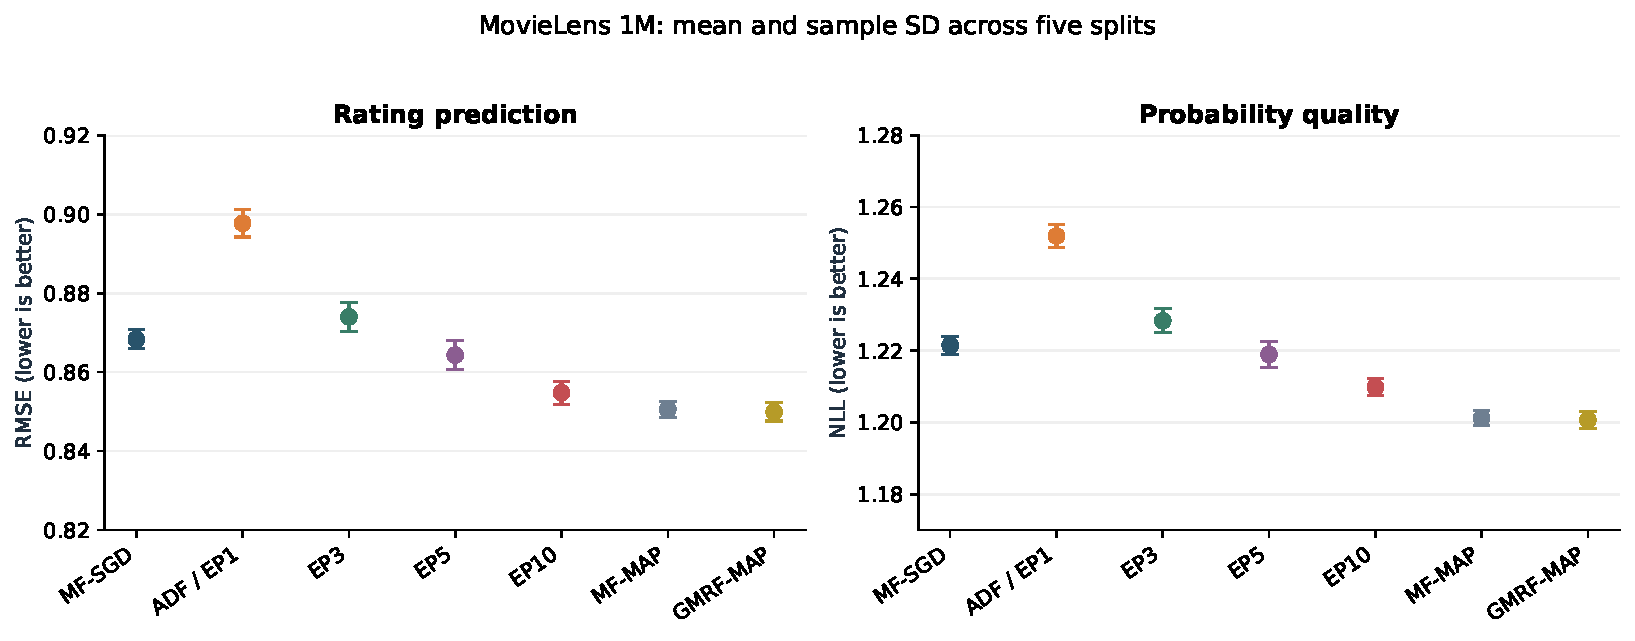
\includegraphics[width=\linewidth]{../../Results/analysis/plots/main_comparison.pdf}
\caption{Accuracy and probability quality. Error bars are sample SD over five
splits, not confidence intervals. The vertical scales are restricted for readability.}
\end{figure}

\subsection{What improvement is actually due to the Markov prior?}
All five clean-validation searches select $\gamma=10$ over 0, 1 and 100.
Against the matching $\gamma=0$ model, the graph reduces mean expected-rating
RMSE by 0.000644 (approximately 0.076\%). The point estimate improves in every
split, but the effect is small in practical star units.

\begin{table}[!htbp]\centering\small
\begin{tabular}{@{}lrr@{}}\toprule
Seed & RMSE reduction & 95\% user-bootstrap interval\\\midrule
42 & +0.000941 & [+0.000562, +0.001330]\\
43 & +0.000380 & [-0.000044, +0.000833]\\
44 & +0.000492 & [+0.000061, +0.000890]\\
45 & +0.000503 & [+0.000070, +0.000937]\\
46 & +0.000906 & [+0.000148, +0.001726]\\
\bottomrule\end{tabular}

\caption{MF-MAP minus GMRF-MAP expected-rating RMSE. Positive means the graph
helps. Intervals use paired user resampling within each fitted split.}
\label{tab:graphci}
\end{table}
Four split-specific intervals lie above zero; seed 43 includes zero. The
conditional bootstrap therefore provides support in several splits without
establishing a universal or independent-replication significance claim.
The NLL difference is also small, and its interval includes zero for several
splits (full table in the results files). We do not claim improved calibration
from the graph: mean ECE changes from 0.03835 to 0.03868, slightly worse.

\begin{figure}[!htbp]\centering
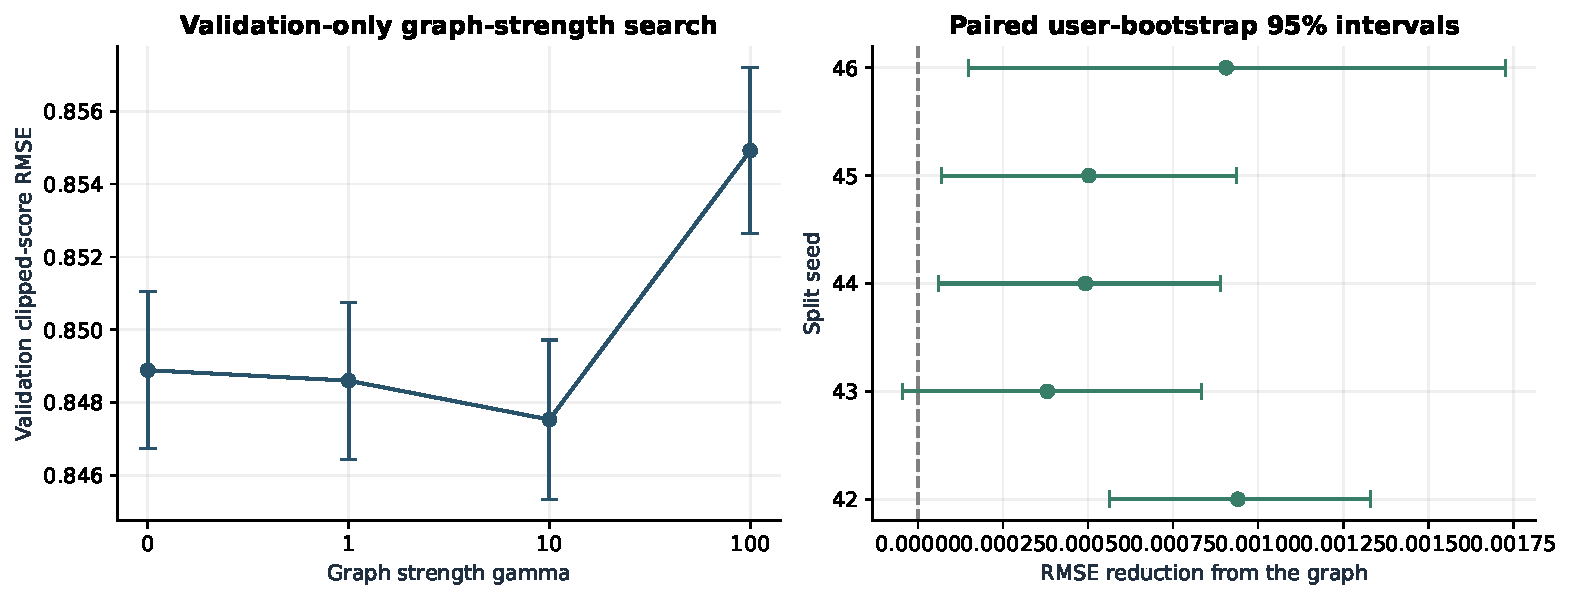
\includegraphics[width=\linewidth]{../../Results/analysis/plots/graph_evidence.pdf}
\caption{Graph-strength validation and the paired graph-only test effect.
Strength 100 worsens validation error; stronger smoothing is not always better.}
\end{figure}

The mechanism is consistent with modest regularization: neighbouring movie
vectors share evidence while the data term retains personalization. The
ablation establishes the effect of this prior \emph{within this solver and
selection protocol}; it does not prove that the selected neighbours are true
dependencies or explain each gain causally. The stress tests below examine
where this explanation remains useful and where it fails.

\subsection{Probability quality and the two noise questions}
\begin{table}[!htbp]\centering\small
\begin{tabular}{@{}lrrr@{}}\toprule
Method & Brier & ECE & Star accuracy\\\midrule
MF-SGD & 0.6554 $\pm$ 0.0011 & 0.0397 $\pm$ 0.0010 & 46.04 $\pm$ 0.16\%\\
ADF / EP1 & 0.6681 $\pm$ 0.0012 & 0.0451 $\pm$ 0.0010 & 44.13 $\pm$ 0.13\%\\
EP3 & 0.6590 $\pm$ 0.0012 & 0.0537 $\pm$ 0.0017 & 45.20 $\pm$ 0.18\%\\
EP5 & 0.6552 $\pm$ 0.0012 & 0.0566 $\pm$ 0.0009 & 45.59 $\pm$ 0.16\%\\
EP10 & 0.6516 $\pm$ 0.0007 & 0.0608 $\pm$ 0.0012 & 46.04 $\pm$ 0.21\%\\
MF-MAP (no graph) & 0.6467 $\pm$ 0.0007 & 0.0383 $\pm$ 0.0018 & 46.98 $\pm$ 0.15\%\\
GMRF-MAP & 0.6468 $\pm$ 0.0009 & 0.0387 $\pm$ 0.0022 & 46.96 $\pm$ 0.19\%\\
\bottomrule\end{tabular}

\caption{Probability quality and exact-star accuracy (percent), five-seed
mean $\pm$ SD. Accuracy uses the most probable star, not rounded expected stars.}
\end{table}
More EP passes improve RMSE, NLL and Brier, but worsen ECE: 0.0451 for ADF,
0.0566 for EP5 and 0.0608 for EP10. Thus lower rating error does not mean more
calibrated confidence. A global empirical distribution has low ECE but poor
personalized error, illustrating that calibration alone is insufficient.
GMRF-MAP has better NLL than EP5/EP10 here, while its probability model still
omits posterior parameter uncertainty. Nominal 90\% equal-tail intervals
cover 98.22\% of ratings for EP5 and 97.41\% for GMRF-MAP, with mean
widths 3.82 and 3.60 star categories. Such broad, discrete intervals should not
be advertised as well calibrated merely because their coverage is high.

\begin{figure}[!htbp]\centering
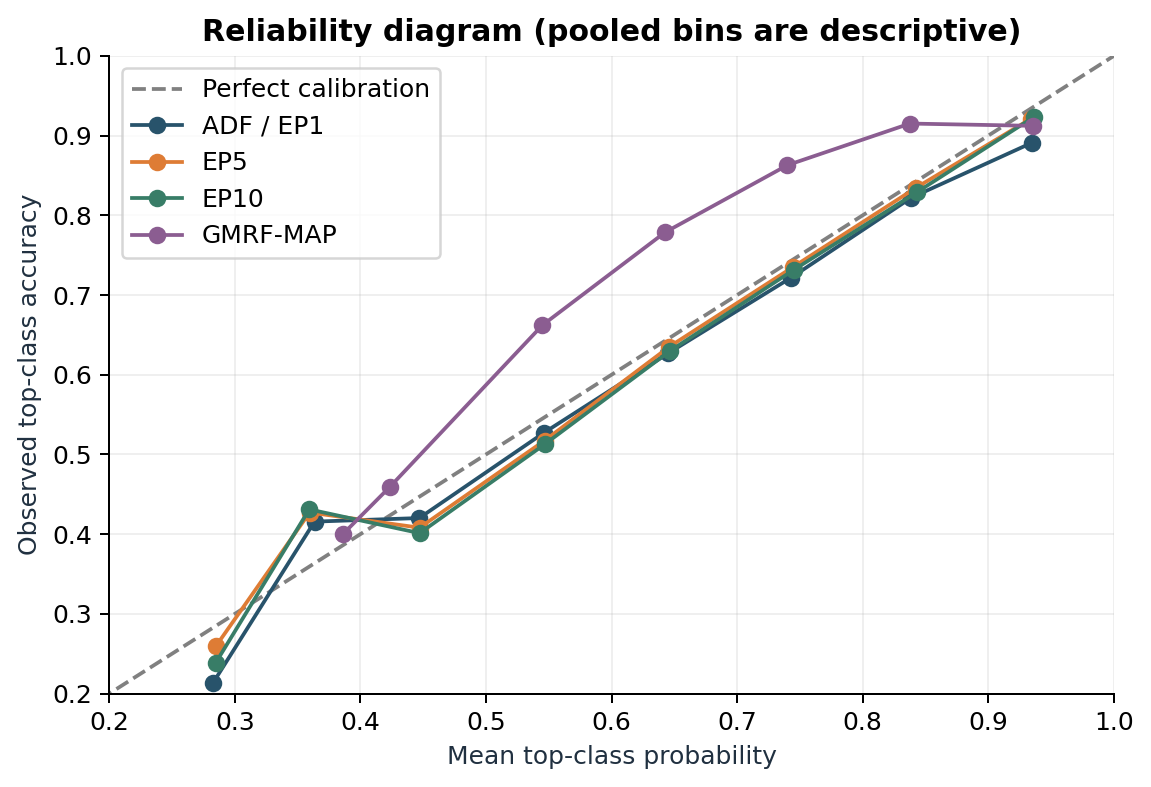
\includegraphics[width=.84\linewidth]{../../Results/analysis/plots/reliability.png}
\caption{Top-class reliability. Pooling overlapping split bins is descriptive;
the curve is not an independent-data significance analysis.}
\end{figure}

\begin{table}[!htbp]\centering\small
\begin{tabular}{@{}lrrr@{}}\toprule
Noise variance & RMSE & NLL & ECE\\\midrule
0.5 & 0.8691 $\pm$ 0.0036 & 1.2404 $\pm$ 0.0054 & 0.0339 $\pm$ 0.0012\\
1.0 & 0.8643 $\pm$ 0.0037 & 1.2189 $\pm$ 0.0035 & 0.0566 $\pm$ 0.0009\\
2.0 & 0.8743 $\pm$ 0.0030 & 1.3154 $\pm$ 0.0020 & 0.0856 $\pm$ 0.0012\\
\bottomrule\end{tabular}

\caption{EP5 observation-noise variance sensitivity. This changes the assumed
likelihood variance, not the dataset's labels.}
\end{table}
Validation NLL chooses $\beta^2=1$ in every seed. Halving it improves ECE to
0.0339 but worsens NLL to 1.2404 and RMSE to 0.8691. Doubling it worsens all
three displayed measures. A smaller assumed variance sharpens probabilities;
the data do not support a blanket claim that reducing noise always improves
inference. The separate label-corruption experiment measures resistance to
wrong training observations while keeping evaluation labels unchanged.

\subsection{Computational cost, convergence and exact-reference checks}
\begin{table}[!htbp]\centering\small
\begin{tabular}{@{}lrrr@{}}\toprule
Method & Fit (s) & Predict ($\mu$s/rating) & Site MiB\\\midrule
MF-SGD & 1.38 $\pm$ 0.04 & 0.413 & 0\\
ADF / EP1 & 3.33 $\pm$ 0.19 & 0.810 & 0\\
EP3 & 10.99 $\pm$ 0.57 & 0.749 & 219.77\\
EP5 & 18.29 $\pm$ 2.02 & 0.679 & 219.77\\
EP10 & 35.99 $\pm$ 6.61 & 0.779 & 219.77\\
MF-MAP (no graph) & 16.74 $\pm$ 2.74 & 0.449 & 0\\
GMRF-MAP & 14.48 $\pm$ 1.82 & 0.487 & 0\\
\bottomrule\end{tabular}

\caption{Selected-candidate fitting and batch prediction cost; mean $\pm$ SD
where shown. EP site memory is an array-size calculation, not process RSS.}
\end{table}
EP5 takes about 5.49 times ADF's mean fit time; EP10 about 10.81 times.
Both repeated-EP budgets use the same 219.77 MiB cache at $K=8$; more passes
increase time rather than site count. MF-SGD fits in about 1.38 seconds under
this implementation. Mean graph construction takes 4.31 seconds and the full
four-candidate MAP search takes 66.37 seconds, beyond the selected GMRF
candidate's 14.48 seconds. A claim that GMRF is simply ``faster than EP'' would
ignore this search/setup cost. Selected MAP wall times vary despite equal epoch
budgets; they do not establish an intrinsic speed advantage from graph edges.

\begin{figure}[!htbp]\centering
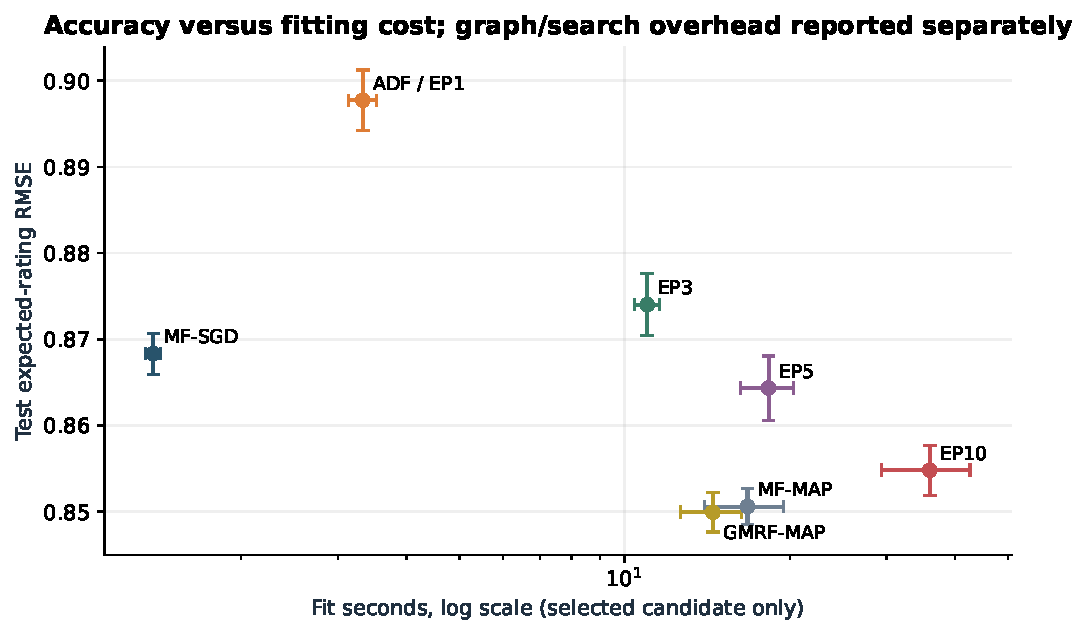
\includegraphics[width=.94\linewidth]{../../Results/analysis/plots/cost_tradeoff.pdf}
\caption{Prediction error versus fitting time. Points omit graph building and
search overhead, which are stated explicitly in the text and raw results.}
\end{figure}

\begin{figure}[!htbp]\centering
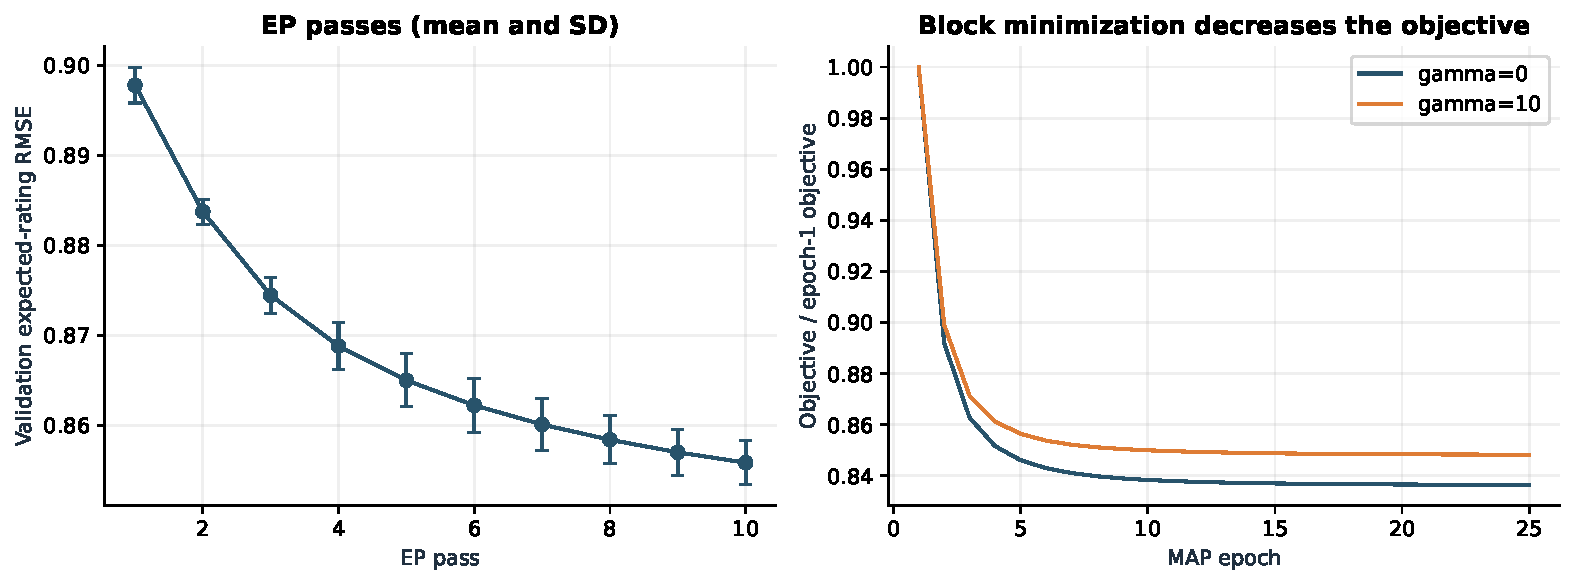
\includegraphics[width=\linewidth]{../../Results/analysis/plots/convergence.pdf}
\caption{Validation error by EP pass and relative MAP objective by epoch.
Lower energy does not guarantee lower held-out error, so validation selects
checkpoints. EP is not claimed to optimize this MAP energy.}
\end{figure}

At EP pass 10, mean RMS parameter change remains 0.01564, despite no skipped
updates in the main EP traces. The local cap is reached by an average of 8.8
updates out of 800,167 at that pass. Stable local calculations therefore do not
establish that the outer posterior approximation has converged.

A separate 12-variable Gaussian Markov diagnostic compares a dense exact
Gaussian solve, Gauss--Seidel MAP iterations and Gibbs sampling. The diagnostic uses a 12-node chain with an extra edge of weight 0.5 between
zero-based nodes 2 and 8, $J=0.8I+2L+\operatorname{diag}(d)$ with $d$
evenly spaced from 0.2 to 1.5, and $h_i=\sin(i+0.4)$.
For $p(q)\propto\exp(-q^TJq/2+h^Tq)$, the known
posterior has mean $J^{-1}h$ and covariance $J^{-1}$. Gauss--Seidel approaches the
exact mean; Gibbs estimates both means and variances with Monte Carlo error.
Increasing sample budget reduces error on average but not necessarily for
every seed. These are additional inference approaches on a tractable
diagnostic, \textbf{not full MovieLens recommender scores}.

\begin{table}[!htbp]\centering\small
\begin{tabular}{@{}lrrrr@{}}\toprule
Method & Budget & Mean RMSE & Variance RMSE & Time (ms)\\\midrule
ExactGaussian & 1 & 0 & 0 & 1.258\\
GaussSeidelMAP & 1 & 0.138 & -- & 0.018\\
GaussSeidelMAP & 5 & 0.00251 & -- & 0.007\\
GaussSeidelMAP & 20 & 4.46e-08 & -- & 0.014\\
GaussSeidelMAP & 100 & 2.17e-17 & -- & 0.066\\
Gibbs & 1000 & 0.0185 & 0.0134 & 2.652\\
Gibbs & 5000 & 0.0111 & 0.00689 & 8.790\\
Gibbs & 20000 & 0.00383 & 0.00333 & 36.379\\
\bottomrule\end{tabular}

\caption{Small Gaussian diagnostic. Gibbs values average five chains/seeds;
1,000 burn-in sweeps are excluded from the sample count but included in time.
MAP has no variance estimate, hence ``--''. Exact/iterative timings are single
small-system measurements. Full variation is in the CSV.}
\end{table}

The original bilinear ordinal quadrature diagnostic is also rerun. It exposes
the same variance/covariance limitations of the factorized approximation;
success on the Gaussian diagnostic does not make bilinear ordinal EP exact.
For a dense $n$-variable Gaussian model, direct solution costs $O(n^3)$,
while a dense iterative or Gibbs sweep costs $O(n^2)$; sparse neighbours
can reduce sweep work. Those guarantees do not turn the full bilinear ordinal
posterior into a Gaussian linear system.

\section{Robustness, ablations and failure analysis}
\subsection{Missing ratings and corrupted observations}
\begin{table}[!htbp]\centering\footnotesize
\begin{tabular}{@{}lrrrr@{}}\toprule
Condition & ADF & EP5 & MF-MAP & GMRF-MAP\\\midrule
main & 0.8980 $\pm$ 0.0049 & 0.8633 $\pm$ 0.0040 & 0.8507 $\pm$ 0.0028 & 0.8501 $\pm$ 0.0031\\
retain\_0.25 & 0.9217 $\pm$ 0.0041 & 0.9199 $\pm$ 0.0051 & 0.9178 $\pm$ 0.0042 & 0.9100 $\pm$ 0.0038\\
retain\_0.5 & 0.9102 $\pm$ 0.0039 & 0.8920 $\pm$ 0.0049 & 0.8810 $\pm$ 0.0039 & 0.8775 $\pm$ 0.0041\\
noise\_0.1 & 0.9129 $\pm$ 0.0036 & 0.8910 $\pm$ 0.0036 & 0.8827 $\pm$ 0.0029 & 0.8797 $\pm$ 0.0030\\
noise\_0.2 & 0.9386 $\pm$ 0.0030 & 0.9326 $\pm$ 0.0022 & 0.9317 $\pm$ 0.0023 & 0.9248 $\pm$ 0.0018\\
cold\_items & 1.0703 $\pm$ 0.0079 & 1.0781 $\pm$ 0.0068 & 1.0622 $\pm$ 0.0060 & 1.0545 $\pm$ 0.0077\\
cold\_users & 0.9837 $\pm$ 0.0137 & 0.9861 $\pm$ 0.0146 & 0.9935 $\pm$ 0.0115 & 0.9916 $\pm$ 0.0117\\
\bottomrule\end{tabular}

\caption{Expected-rating test RMSE, mean $\pm$ sample SD over seeds 42--44.
The clean row uses these same three seeds. Cold-start rows evaluate different
restricted test populations and should not be ranked directly against the clean row.}
\end{table}

Reducing training availability increases error for all methods. At 25\%
retention, the graph reduces MF-MAP RMSE from 0.9178 to 0.9100; at 50\%,
from 0.8810 to 0.8775. The corresponding gains, 0.0077 and 0.0036, are larger
than the clean three-seed gain of 0.0006. Sharing evidence is more useful when
each movie has less direct support. This supports the variance-reduction
hypothesis under random removal, while not establishing robustness to actual
nonrandom exposure or missing-not-at-random ratings.

With 10\% corrupted labels, MF-MAP and GMRF-MAP have RMSE 0.8827 and 0.8797;
at 20\%, 0.9317 and 0.9248. The graph mitigates some degradation but does not
recover clean-data performance. Both the training target and the residual
similarities are affected by corruption. The graph helps here despite that
imperfect evidence, consistent with useful smoothing; this experiment does
not identify a universally optimal graph or realistic user-error mechanism.

EP5 remains better than ADF in aggregate, but its advantage becomes small
under sparse or heavily corrupted training. At 25\% retention, seed 43's EP5
is slightly worse than ADF. Repeated inference cannot create reliable evidence
that is absent and may reinforce misspecified observations. These stress
comparisons are descriptive three-seed results, not independent-dataset
significance tests.

\begin{figure}[!htbp]\centering
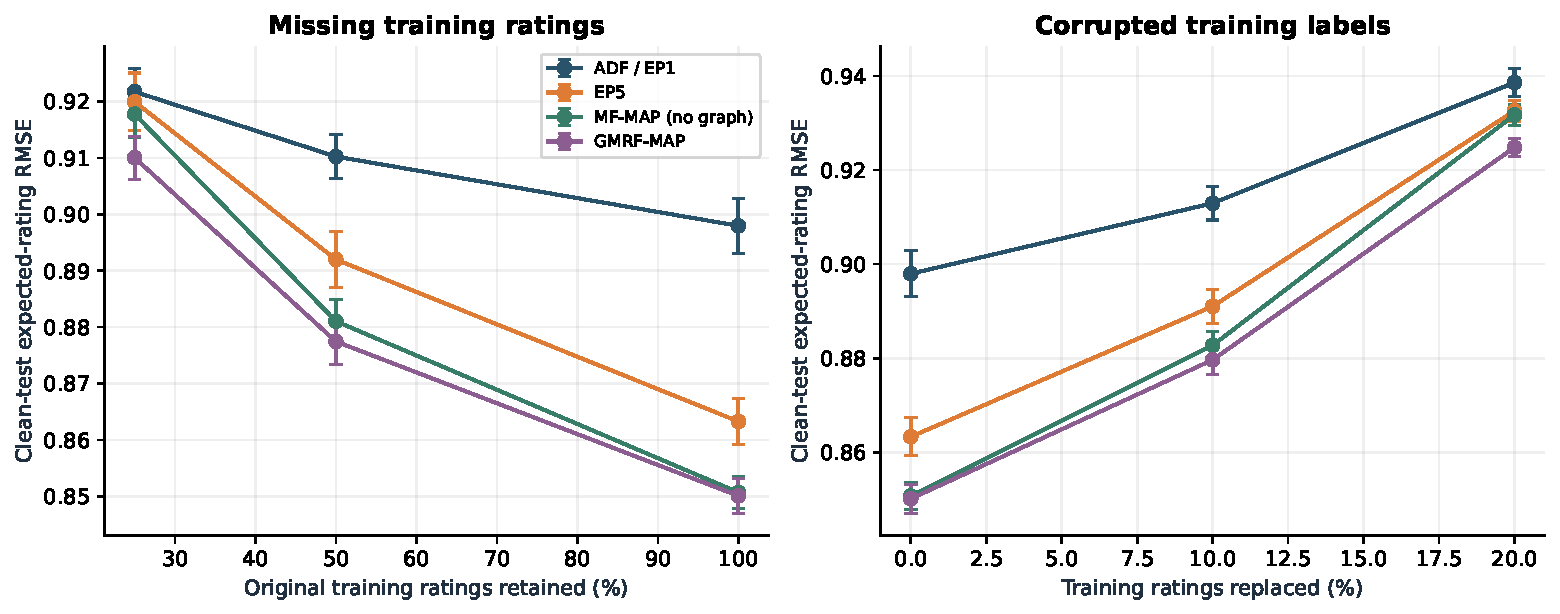
\includegraphics[width=\linewidth]{../../Results/analysis/plots/robustness.pdf}
\caption{Missing-data and label-noise sensitivity. All evaluations use clean
test labels; error bars show sample SD across the same three seeds.}
\end{figure}

\subsection{Which graph components matter?}
\begin{table}[!htbp]\centering\small
\begin{tabular}{@{}lrr@{}}\toprule
Graph condition & MF-MAP RMSE & GMRF-MAP RMSE\\\midrule
main & 0.8507 $\pm$ 0.0028 & 0.8501 $\pm$ 0.0031\\
ratings\_only & 0.8507 $\pm$ 0.0028 & 0.8499 $\pm$ 0.0031\\
genres\_only & 0.8507 $\pm$ 0.0028 & 0.8510 $\pm$ 0.0031\\
graph\_top\_5 & 0.8507 $\pm$ 0.0028 & 0.8497 $\pm$ 0.0031\\
graph\_top\_50 & 0.8507 $\pm$ 0.0028 & 0.8505 $\pm$ 0.0031\\
\bottomrule\end{tabular}

\caption{Graph ablations at fixed $\gamma=10$, three seeds. The graph-free
baseline is unchanged across clean graph variants.}
\end{table}
Ratings-only edges give mean RMSE 0.8499, mixed edges 0.8501, and genre-only
edges 0.8510, versus 0.8507 without a graph. Thus coarse genres alone do not
improve this warm-interaction benchmark. They can connect movies whose
audiences or rating patterns differ; adding metadata is not automatically
beneficial. Genre information still supplies connections for unseen items,
which is a different evaluation setting.

Top-5 neighbours give RMSE 0.8497, whereas top-50 gives 0.8505. More edges do
not necessarily carry more useful information. Combined with the poorer
validation result at strength 100, this reveals an oversmoothing risk.
These topology variants are exploratory diagnostics. The main configuration
remains top-20, fixed before these test comparisons; we do not select a new
reported winner using their test scores.

\subsection{Controlled cold-start and remaining errors}
For withheld movies, GMRF-MAP improves the matching baseline from 1.0622 to
1.0545 RMSE. Genre connections can transfer neighbouring traits when a movie
has no training observations, but its own rating bias cannot be estimated.
Error remains much higher than on the warm main benchmark. EP5 is worse than
ADF here (1.0781 versus 1.0703), another counterexample to universal EP
superiority.

For withheld users, ADF has RMSE 0.9837, EP5 0.9861, MF-MAP 0.9935 and
GMRF-MAP 0.9916. The movie graph offers no user metadata or user-specific
evidence, so it cannot personalize a completely unseen user. It slightly helps
its matching MAP baseline but does not beat ADF in this setting. This limits
the claim that a movie network resolves cold-start in general.

\begin{figure}[!htbp]\centering
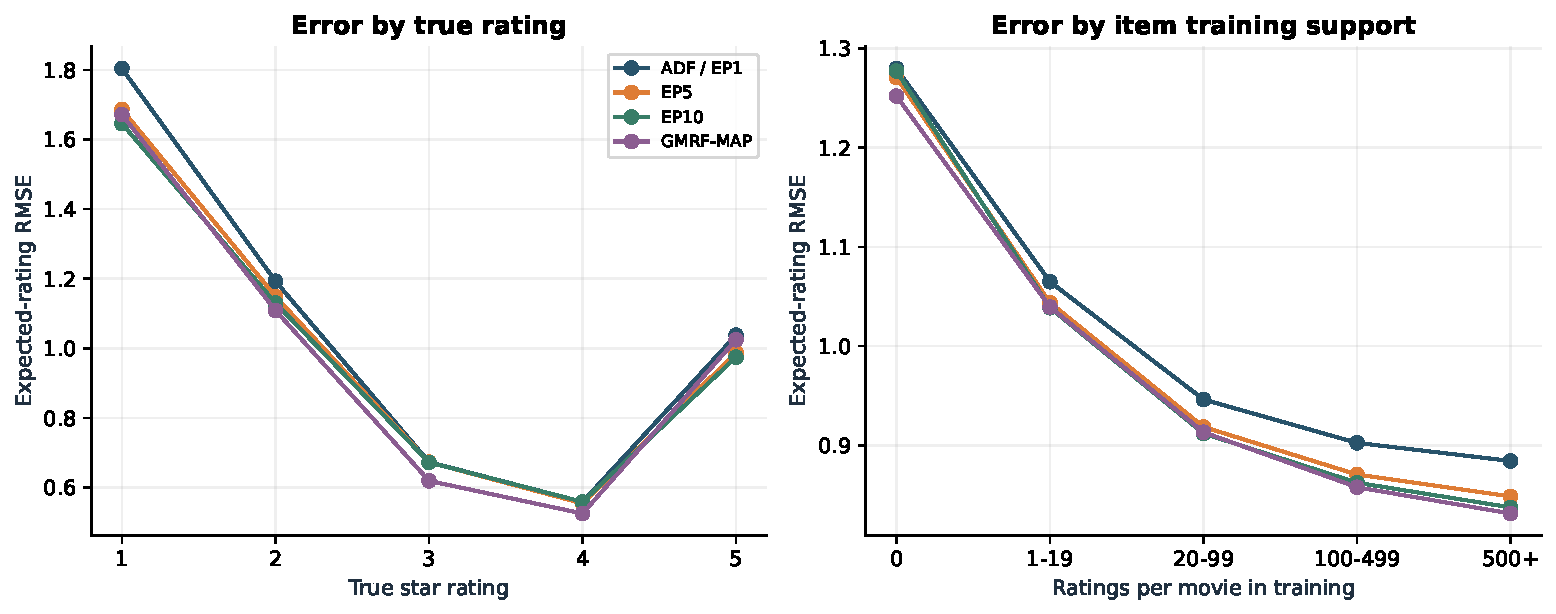
\includegraphics[width=\linewidth]{../../Results/analysis/plots/error_analysis.pdf}
\caption{Descriptive pooled errors by true rating and movie support. Pooled
split observations overlap; the curves do not represent independent samples.}
\end{figure}

The main benchmark's five-star error is 1.0245 for GMRF-MAP versus 0.9748 for
EP10, despite GMRF's better aggregate RMSE. Its advantages are stronger around
three/four-star observations. The expected-rating decision and regularization
shrink predictions toward the centre, overpredicting low ratings and
underpredicting high ratings. An overall score therefore hides meaningful
class-specific failures.

Low-support movies are harder for every method. The natural zero-training-item
bin contains only 83 pooled test observations across five overlapping splits;
its curve should not support a broad cold-start claim. The controlled
withheld-item experiment is the more appropriate evidence. Support strata
also differ in movie composition, so their error differences are descriptive,
not causal estimates of adding ratings.

\subsection{Prior, damping and order sensitivity}
\begin{table}[!htbp]\centering\small
\begin{tabular}{@{}lrr@{}}\toprule
EP5 variant & RMSE & NLL\\\midrule
ADF\_reshuffled & 0.8984 $\pm$ 0.0049 & 1.2526 $\pm$ 0.0046\\
damping\_0.25 & 0.8752 $\pm$ 0.0048 & 1.2292 $\pm$ 0.0041\\
damping\_1 & 0.8529 $\pm$ 0.0038 & 1.2078 $\pm$ 0.0027\\
prior\_0.1 & 0.8672 $\pm$ 0.0043 & 1.2216 $\pm$ 0.0036\\
prior\_0.5 & 0.8650 $\pm$ 0.0039 & 1.2195 $\pm$ 0.0031\\
reshuffled & 0.8638 $\pm$ 0.0039 & 1.2183 $\pm$ 0.0030\\
\bottomrule\end{tabular}

\caption{Fixed EP5 sensitivity variants, mean $\pm$ SD over seeds 42--44.
Each varies one operating choice; the main configuration is not reselected
using these test outcomes. Reshuffled ADF is the first pass of that order.}
\end{table}
Prior strength changes regularization, damping changes the size of cached-site
replacements, and reshuffling changes the sequence of approximate updates.
These comparisons expose dependence on operating choices rather than proving
that the original settings are optimal. Their validation trajectories and
test metrics are supplied together. A broader validation-only search would
be needed to compare optimized method families fairly; this finite study
does not claim exhaustive tuning or order invariance.

With undamped replacement after the first pass (outer damping 1), EP5 reaches
mean RMSE 0.8529 across the three sensitivity seeds, compared with 0.8633 for
the original EP5 setting and 0.8501 for GMRF-MAP on those same seeds.
Thus tuning the inference schedule closes much of the apparent gap. This is
an exploratory fixed-variant comparison, not a validation-selected replacement
for the five-seed main method. It further limits any claim that graph structure
alone explains superior performance.


\section{Related work and revised SOTA positioning}
\textbf{Matchbox: Microsoft Research, WWW 2009.} Stern, Herbrich and
Graepel~\cite{stern2009} combine latent features, optional metadata, feedback
models and hybrid message passing. ADF provides efficient online Bayesian
updates; repeated EP revisits cached rating contributions. Their experiments
study recommendation accuracy, cold-start behaviour and scalability. Our
implementation retains the inference question but uses static ID features,
fixed cuts and its own schedule, rather than reproducing Infer.NET or the full
system. Published scores use different protocols and are not directly comparable.

\textbf{PreRec: AWS AI Labs affiliation, WSDM 2024.} Lin et al.~\cite{lin2024}
use a hierarchical Bayesian model with neural user/item encoders, domain
variables and popularity effects. Training uses MAP optimization;
zero-shot scoring changes domain and popularity mechanisms. XMarket/Online
Retail experiments evaluate cross-domain sequential ranking and limited-data
adaptation with Recall and revised NDCG metrics. Reported gains support modelling transfer and bias in that setting,
subject to the learned representations and assumed bias mechanisms. They do
not establish an EP advantage or provide a MovieLens rating baseline.

The evidence revises our position from an implementation comparison to a
controlled inference-and-regularization study. Longer EP passes improve
prediction at extra time and imperfect calibration. A GMRF adds a small
benefit over an already strong MAP baseline; robustness experiments limit
any claim of general superiority. The implemented contributions are comparative
experiments, mathematical checks and interpretation, not a new inference
algorithm or causal-debiasing system. Neither published paper's scores are
numerically compared with ours because the evaluation protocols differ.

\section{Limitations and conclusion}
The model is static and evaluated through random interactions, not future
recommendations. Learned latent coordinates are not uniquely identifiable
semantic traits. EP retains a factorized approximation and cannot represent
all posterior correlations. Its moment and convergence checks validate
specific properties rather than global exactness. GMRF-MAP uses point
estimates, and its fitted residual scale does not recover Bayesian parameter
uncertainty. Similarity edges can be wrong, particularly under sparse or
corrupted observations; neither genres nor correlations establish causality.

The parameter searches are finite and not an exhaustive optimum comparison.
Several selected checkpoints reach the budget boundary. SGD and MAP have
different regularization conventions, and the EP/MAP likelihoods differ.
Changing them jointly is useful for a system comparison but does not isolate
the graph. Confidence intervals are conditional on fitted models and resample
users only; overlapping splits and shared-item dependence restrict the scope
of significance claims. Missingness/corruption are controlled artificial stress
mechanisms, not a full model of actual user reporting or exposure bias.

M3 answers the M2 feedback with multiple fitting/inference approaches, a
mathematically specified Markov network, matched ablations, explicit noise
experiments, probability-quality measures and statistical interpretation.
On the main benchmark, GMRF-MAP's RMSE is $0.8499\pm0.0023$, versus
$0.8643\pm0.0037$ for EP5 and $0.8548\pm0.0029$ for EP10. The comparison that
isolates the graph is much closer: $0.8506\pm0.0021$ without it versus
$0.8499\pm0.0023$ with it. The observed graph gain is therefore modest,
with split-dependent statistical support, while its benefit is more visible
in some stress conditions.

The defensible explanation is that the pairwise prior can share evidence
between related movies and reduce estimation variance, while excessive or
unhelpful connections introduce bias. This mechanism and the matched ablation
support a qualified improvement claim; they do not imply that any Markov or
Bayesian network will improve any recommender. Repeated EP likewise improves
prediction without uniformly improving calibration. The project's contribution
is the reproducible evidence about these trade-offs and limitations.

Next steps are learned user-specific thresholds, chronological evaluation,
better treatment of nonrandom missingness, broader validation-only tuning,
and a posterior approximation that retains graph-related covariance. These
are proposed extensions, not completed experiments or claims in this submission.


\FloatBarrier
\bibliographystyle{plain}
\bibliography{references}
\clearpage
\appendix
\section{Requirement coverage and report continuity}
Table~\ref{tab:coverage} maps the M3 expectations in the CSE 516 project
guidelines to the evidence in this report and repository.

\begin{table}[!htbp]\centering\small
\begin{tabularx}{\linewidth}{@{}lX@{}}\toprule
M3 expectation & Evidence in the cumulative report/package\\\midrule
Full experimental results & Five main seeds; three stress-test seeds; raw metrics and configs\\
Baseline comparison & M2 means/SGD/ADF/EP; graph-free MAP and matching GMRF\\
KPI plots and tables & Rating/probability errors, cost, reliability, convergence, stress and errors\\
Variation and uncertainty & Sample SD; 2,000-replicate paired user-bootstrap intervals with limits\\
Probability quality & NLL, Brier, ECE, reliability and interval outputs\\
Robustness & Training availability, label corruption, assumed noise, graph density, cold items/users\\
Ablation and error analysis & Gamma=0, genre/residual components, rating/support groups\\
Interpretation & Main-result explanations, counterexamples and explicit attribution limits\\
Theoretical validation & Preserved EP derivation; proper GMRF prior; exact/Gibbs/iterative diagnostic; quadrature\\
Revised SOTA position & Specific Matchbox/PreRec models and protocols; no direct SOTA score claim\\
Reproducibility & Source/config/environment hashes, run logs, tests, result/figure scripts\\
Team roles & Member responsibilities listed in the team section below\\\bottomrule
\end{tabularx}
\caption{Coverage of the M3 guidelines. SHD is inapplicable without a true graph.}\label{tab:coverage}
\end{table}

The updated source begins from the revised M2 \code{main.tex} and preserves its
title, team details, model equations, EP/VMP derivation and numerical-validation
discussion. It updates the abstract, milestone/date, benchmark, results,
positioning and conclusion; it adds the GMRF representation and M3 analysis.
A detailed M2-to-M3 changelog is in \code{Review/CHANGELOG\_M2\_TO\_M3.md}.

Not every item mentioned as possible future work in M2 is claimed complete.
The implemented additions cover noise/prior/damping/order sensitivity, longer
EP runs, genre ablations, reduced data and cold-start evaluations. Learned
user-specific thresholds, a temporal deployment test, and full-posterior GMRF
inference remain deferred. The formal general guidelines encourage depth in
one question, rather than an unsupported claim to have tested every PGM method.

\section{Team accountability and AI assistance}
Team roles follow the M1/M2 plan: Jyotier Vithalani (AU2440170): mathematical
model, EP/ADF and repository; Tanmay Kanani (AU2440234): baselines; Ansh
Chaudhari (AU2440259): paper/SOTA analysis; Shlok Shah (AU2440178): dataset and
metadata; Het Patel (AU2440221): KPIs, experiment tracking and documentation.

Generative AI assisted implementation, execution, analysis and writing. All
numerical results were computed by the included code on the verified dataset;
team members remain responsible for checking them.

\section{Reproduction and evidence boundaries}
Code, configurations and results are in the
\code{M3\_g4\_th\_apl\_recommend-sys\_team} folder of the project repository.
The Code README provides commands for validation, main/stress/sensitivity
experiments, figure regeneration and report compilation. Raw MovieLens files
are not redistributed; the official downloader, source links and hashes are
included. Seed-42 checkpoints and ID mappings support direct probability queries.

The main-run source snapshot and its hashes preserve the exact executed
implementation. Later changes add a cold-user condition and audit metadata to
the robustness path, without changing the main numerical kernels or selection
rules. Results from the separate main, robustness and sensitivity stages retain
their individual configurations and source/environment records.

The earlier synthetic offline demo is excluded from all MovieLens benchmark
tables. The 12-variable Gaussian example is labelled a diagnostic throughout.
Historical M2 files are labelled separately. Training time excludes JIT and
test evaluation; comparison of complete workflows additionally includes graph
construction and validation search. Test evaluation follows validation selection
for each comparison.

\end{document}
